X-ray binaries are a class of binary star system that are luminous in X-rays. 
They consist of a compact object, \textbf{either a neutron star or a black hole}, which is accreting matter from a companion star. These systems are crucial astrophysical laboratories, as they provide the primary means of discovering and measuring the mass of stellar-mass black holes, allowing us to probe the limits of physics in extreme gravitational fields.

\section{Classification of XRBs}

The primary classification of X-Ray Binaries is based on the \textbf{mass of the companion star} (the secondary) in the binary. We break these down into three groups:
\par
\vspace{10pt}
\begin{enumerate}
    \item \textbf{Low-Mass X-Ray Binaries (LMXBs)}: These are the most common type of X-ray binary in the galaxy. They are old systems, typically found in the galactic bulge and halo. The companion is a star with mass less than $\sim 1 M_{\odot}$. The donor is a late-type, evolved star like a red giant or a main-sequence star similar to our sun. The primary mechanism for these types of binaries is \textbf{Roche-Lobe overflow}. This mechanism has a \textbf{tendency to make LMXBs transient.}


    \item \textbf{Intermediate-Mass X-Ray Binaries (IMXBs)}: A relatively rare and less well-defined class that bridges the gap between LMXBs and HMXBs. In the intermediate range, typically $\sim 1-10 M_{\odot}$. The donor is usually a B or A-type star. The mechanism can be complex and depends on the evolutionary stage. It can begin as a weak stellar wind, but as the star evolves and expands, it will transition to Roche Lobe Overflow. This process is generally unstable and very rapid.

    \item \textbf{High-Mass X-Ray Binaries (HMXBs)}: These are young systems, typically found in the star-forming regions of the galactic disk. Greater than $\sim 10 M_{\odot}$. The donor is a young, massive, and luminous O or B-type supergiant star. Occurs primarily through a strong, high-velocity \textbf{stellar wind} from the massive companion. The compact object's gravity captures a small fraction of this outflowing wind via Bondi-like accretion. These are less frequently transient than LMXBs.
\end{enumerate}
\vspace{10pt}
\section{Low Mass XRBs}
\begin{figure}[ht!]
    \centering
    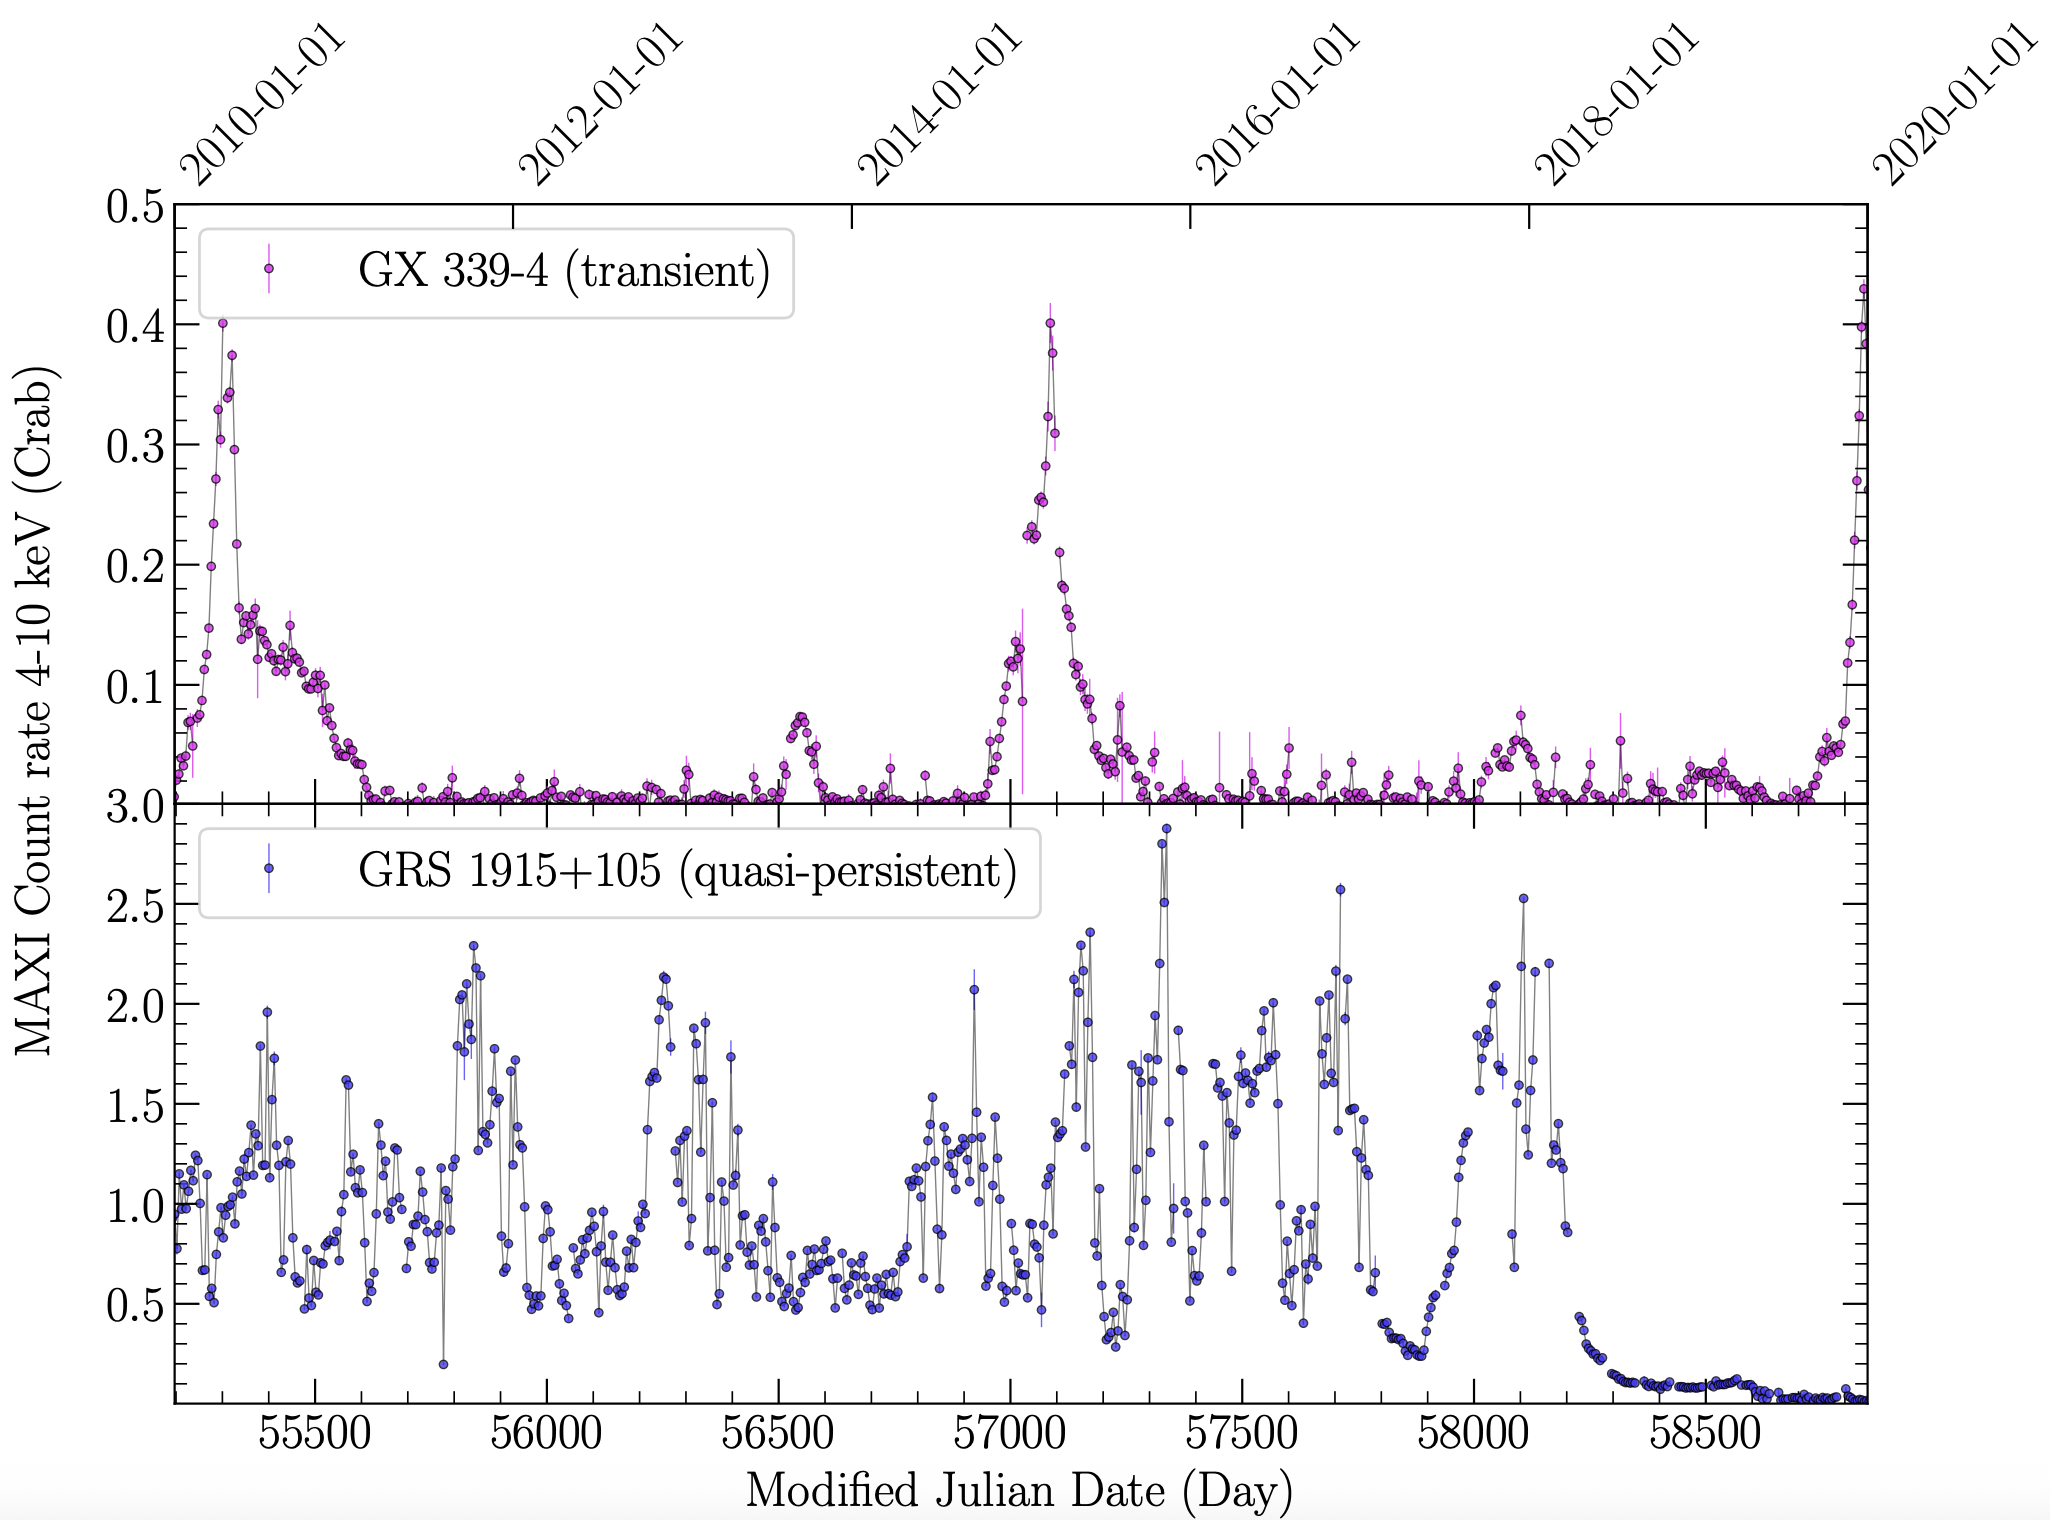
\includegraphics[width=0.75\linewidth]{Pictures/figures/lmxb_lcurves.png}
    \caption{Light curves of LMXBs and their variability over the past decade based on monitoring data from MAXI/GSC. Top: The transient black hole LMXB GX339-4, showing several distinct accretion outbursts of different brightness. Bottom: The quasi-persistent black hole LMXB GRS 1915+105, illustrating that large variations in brightness can also occur in systems that are continuously active.}
    \label{fig:placeholder}
\end{figure}
Low-Mass X-ray Binaries (LMXBs) are primarily characterized by their \textbf{phenomenological behavior}, meaning the observable changes in their emission over time. A significant population of these systems are so-called \textbf{soft X-ray transients} or \textbf{X-ray novae}. These LMXBs exhibit dramatic outbursts separated by long periods of quiescence, although other systems can display quasi-persistent X-ray emission (see Figure X).

The fundamental difference between transient and persistent behavior lies in the \textbf{stability of the accretion disk}. If the mass transfer rate from the companion star is sufficiently high, the disk remains hot and ionized, leading to stable accretion and persistent X-ray emission. However, if the rate falls below a critical threshold, the disk becomes unstable, resulting in a cycle of long quiescent phases punctuated by brief, luminous outbursts.

The \textbf{quiescent phase} is of immense astrophysical value. During this period, the accretion disk is extremely dim, allowing for unobscured observation of the companion star, which is best done in optical bands. This provides a crucial window to characterize the binary system by studying details in the star's light curve. Most importantly, we can observe the periodic \textbf{ellipsoidal variations} caused by the tidal distortion of the companion star as it orbits, which is essential for determining the system's inclination and, ultimately, the mass of the compact object.

\subsection{Spectroscopic Characteristics and States}

\begin{figure}[ht!]
    \centering
    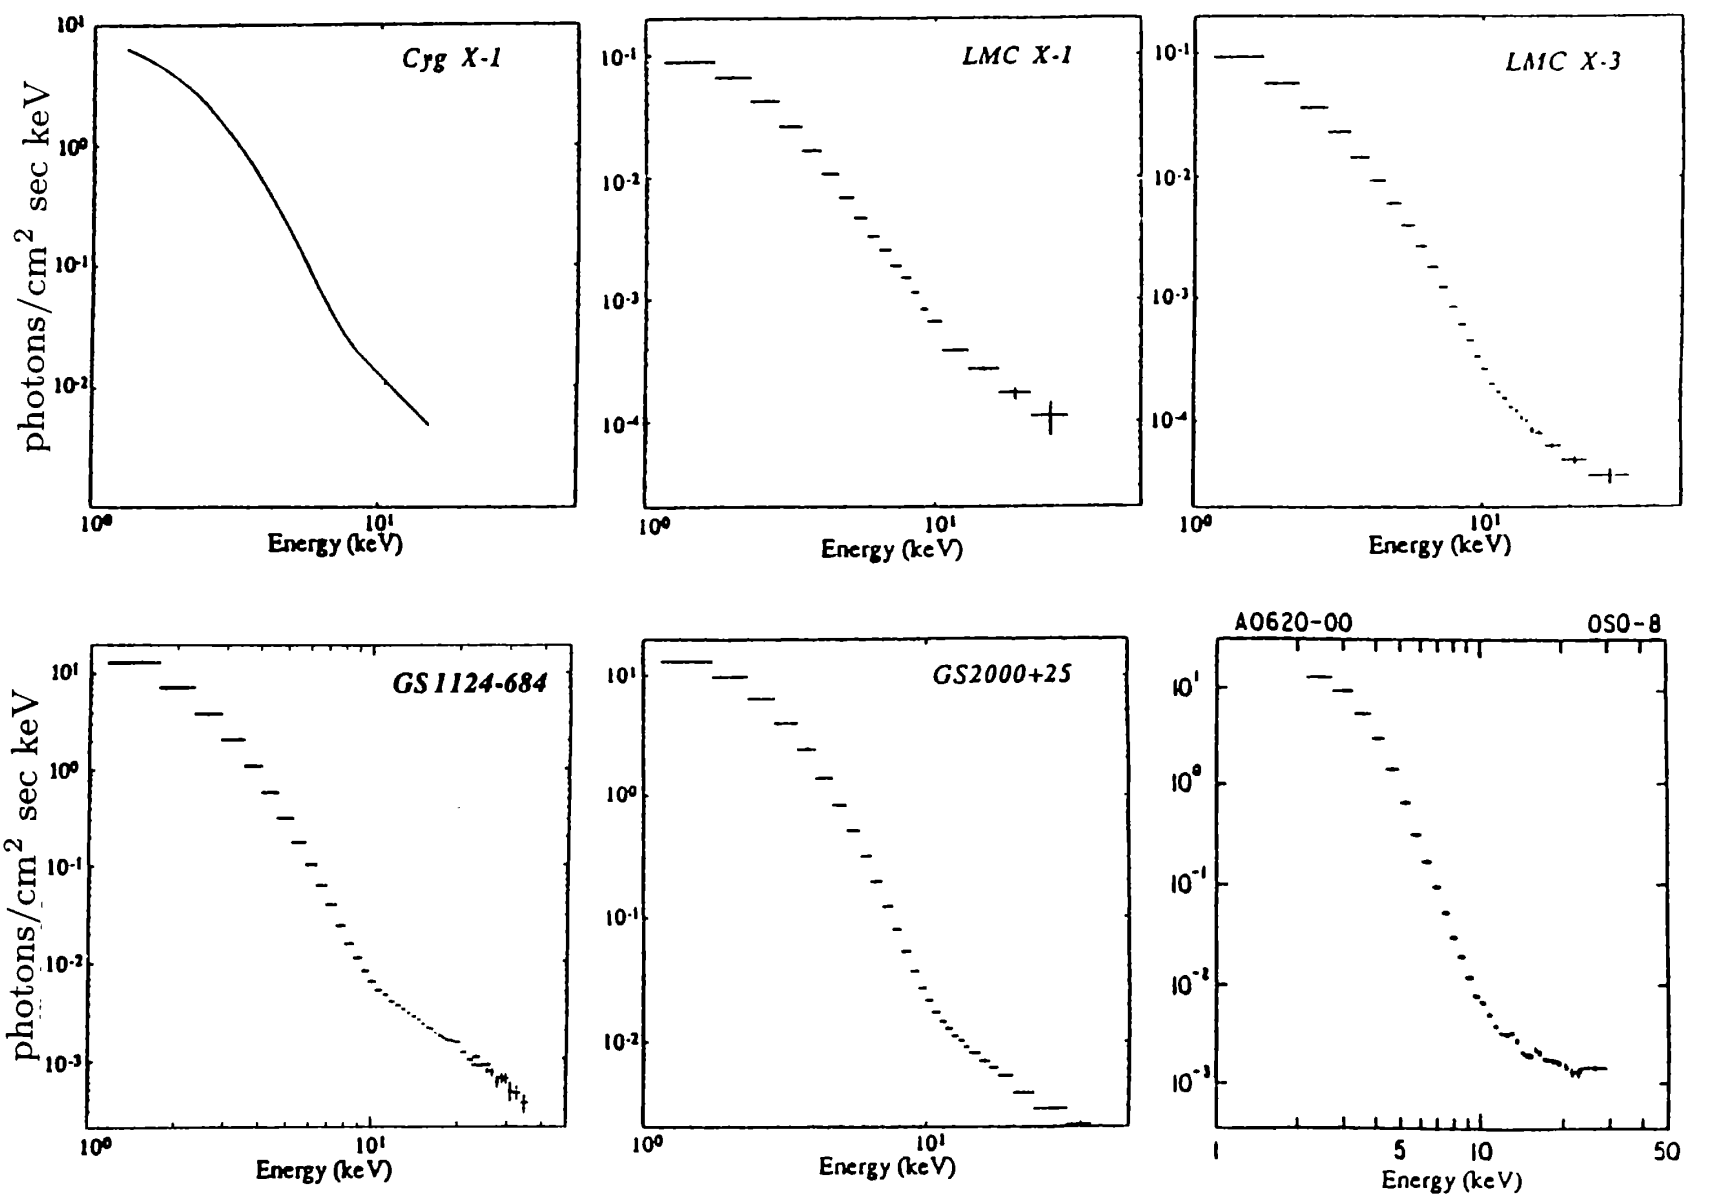
\includegraphics[width=0.75\linewidth]{Pictures/figures/lmxb_spectra.png}
\caption{A model of a typical X-ray spectrum for a Low-Mass X-ray Binary. The total observed spectrum (solid black line) is a composite of several physical components. The dominant thermal emission from the accretion disk is modeled as a \textbf{disk blackbody} (blue curve), which characterizes the bright, High/Soft State. In contrast, the \textbf{Low/Hard State} is dominated by a non-thermal power-law produced by \textbf{Comptonization} (red dashed line) in a hot corona. Additionally, hard X-rays from the corona can reflect off the surface of the accretion disk, producing a \textbf{reflection} component (green dotted line) which includes features like the relativistically broadened iron line.}
\end{figure}

The X-ray spectrum of an LMXB is not static; it provides a rich diagnostic of the accretion flow, which changes dramatically depending on the system's state. While thermal emission is a key component, the full spectrum reveals a more complex picture involving non-thermal processes and the effects of general relativity. LMXBs primarily exhibit two distinct spectral states:
\vspace{10pt}
\begin{itemize}
    \item \textbf{The High/Soft State:} During the peak of an outburst, the spectrum is dominated by strong, soft thermal emission from the accretion disk. This is not a single blackbody, but rather a \textbf{multi-temperature blackbody spectrum} arising from the temperature gradient across the disk, with the inner regions being the hottest. Fitting this thermal continuum allows astronomers to estimate the temperature and apparent inner radius of the disk, a technique which is foundational to measuring black hole spin.

    \item \textbf{The Low/Hard State:} Observed during quiescence and at the beginning and end of outbursts, this state is characterized by a much harder spectrum. The thermal emission from the disk is weak or absent. Instead, the spectrum takes the form of a \textbf{non-thermal power-law} that can extend to very high energies ($>100$ keV). This emission is understood to be the result of \textbf{Comptonization}, where soft photons are up-scattered by a corona of hot, energetic electrons surrounding the central object.
\end{itemize}
\vspace{10pt}
Beyond the continuum, LMXB spectra can display profound signatures of the extreme physics near the compact object. The most significant of these is the \textbf{relativistically broadened iron K$\alpha$ line}. While iron in the accreting gas is expected to produce a narrow emission line at 6.4 keV, the immense gravity and orbital velocity near a black hole warp its appearance. The line is smeared out by Doppler effects from the disk's rotation (approaching the speed of light) and skewed to lower energies by gravitational redshift. Modeling the precise shape of this broad iron line provides a direct probe of the innermost stable circular orbit, and is one of the primary methods used to measure the \textbf{spin of the black hole}.

\par

The journey of an LMXB through an outburst cycle is best understood as a progression through distinct accretion states, each with a unique physical geometry and a corresponding set of observational signatures. These states can be tracked using a Hardness-Intensity Diagram (HID), which maps the evolution of the X-ray spectrum and its connection to the launching of relativistic jets.
\vspace{10pt}
\begin{enumerate}

    \item \textbf{The Low/Hard State (LHS):} This is the state where the system resides during quiescence and at the beginning of an outburst.
    \begin{itemize}
        \item \textbf{Physical Nature:} The accretion flow is characterized by a cool, geometrically thin accretion disk that is truncated at a large distance from the black hole. The inner region is dominated by a hot, geometrically thick, and optically thin \textbf{corona}.
        \item \textbf{Observational Signatures:}
        \begin{itemize}
            \item \textbf{X-ray Spectrum:} The spectrum is dominated by a hard, non-thermal \textbf{power-law} produced by the Comptonization of soft photons in the hot corona. The thermal emission from the cool outer disk is very weak or absent.
            \item \textbf{Radio Emission:} A steady, compact \textbf{relativistic jet} is consistently active in this state, making the system a "microquasar."
            \item \textbf{Variability:} The X-ray emission exhibits strong, rapid, aperiodic variability (flickering) on short timescales.
            \item \textbf{Location on HID:} Occupies the right-hand branch of the HID, characterized by high hardness and low-to-medium intensity.
        \end{itemize}
    \end{itemize}

    \item \textbf{The High/Soft State (HSS):} This is the state the system transitions into near the peak of its outburst.
    \begin{itemize}
        \item \textbf{Physical Nature:} The structure of the accretion flow changes dramatically. The hot corona shrinks or disappears, and the cool, geometrically thin, and optically thick accretion disk extends all the way down to the black hole's \textbf{Innermost Stable Circular Orbit (ISCO)}.
        \item \textbf{Observational Signatures:}
        \begin{itemize}
            \item \textbf{X-ray Spectrum:} The spectrum is now dominated by soft, thermal emission. It is well-modeled as a \textbf{multi-temperature disk blackbody}, representing the combined emission from different radii of the hot inner disk.
            \item \textbf{Radio Emission:} The steady, compact jet is \textbf{quenched} or completely shut off in this state.
            \item \textbf{Variability:} The rapid X-ray variability is strongly suppressed; the emission is much more stable.
            \item \textbf{Location on HID:} Occupies the lower-left branch of the HID, characterized by low hardness and the highest intensity.
        \end{itemize}
    \end{itemize}

    \item \textbf{The Intermediate States:} These are the short-lived, complex phases that occur as the system transitions between the LHS and HSS.
    \begin{itemize}
        \item \textbf{Physical Nature:} The geometry of the accretion flow is in flux, with the inner edge of the thin disk moving inwards (during the hard-to-soft transition) or outwards (during the soft-to-hard transition).
        \item \textbf{Observational Signatures:}
        \begin{itemize}
            \item \textbf{X-ray Spectrum:} The spectrum shows a mixture of both strong thermal disk emission and a significant hard power-law tail from the Comptonizing corona.
            \item \textbf{Radio Emission:} These states are often associated with major, discrete jet ejections. As the system transitions from hard to soft, it can launch a powerful, transient blob of plasma before the steady jet fully quenches.
            \item \textbf{Location on HID:} Occupy the top, horizontal track of the HID, connecting the two main branches.
        \end{itemize}
    \end{itemize}
\end{enumerate}
\vspace{10pt}
\section{High Mass XRBs}

\begin{figure}[ht!]
    \centering
    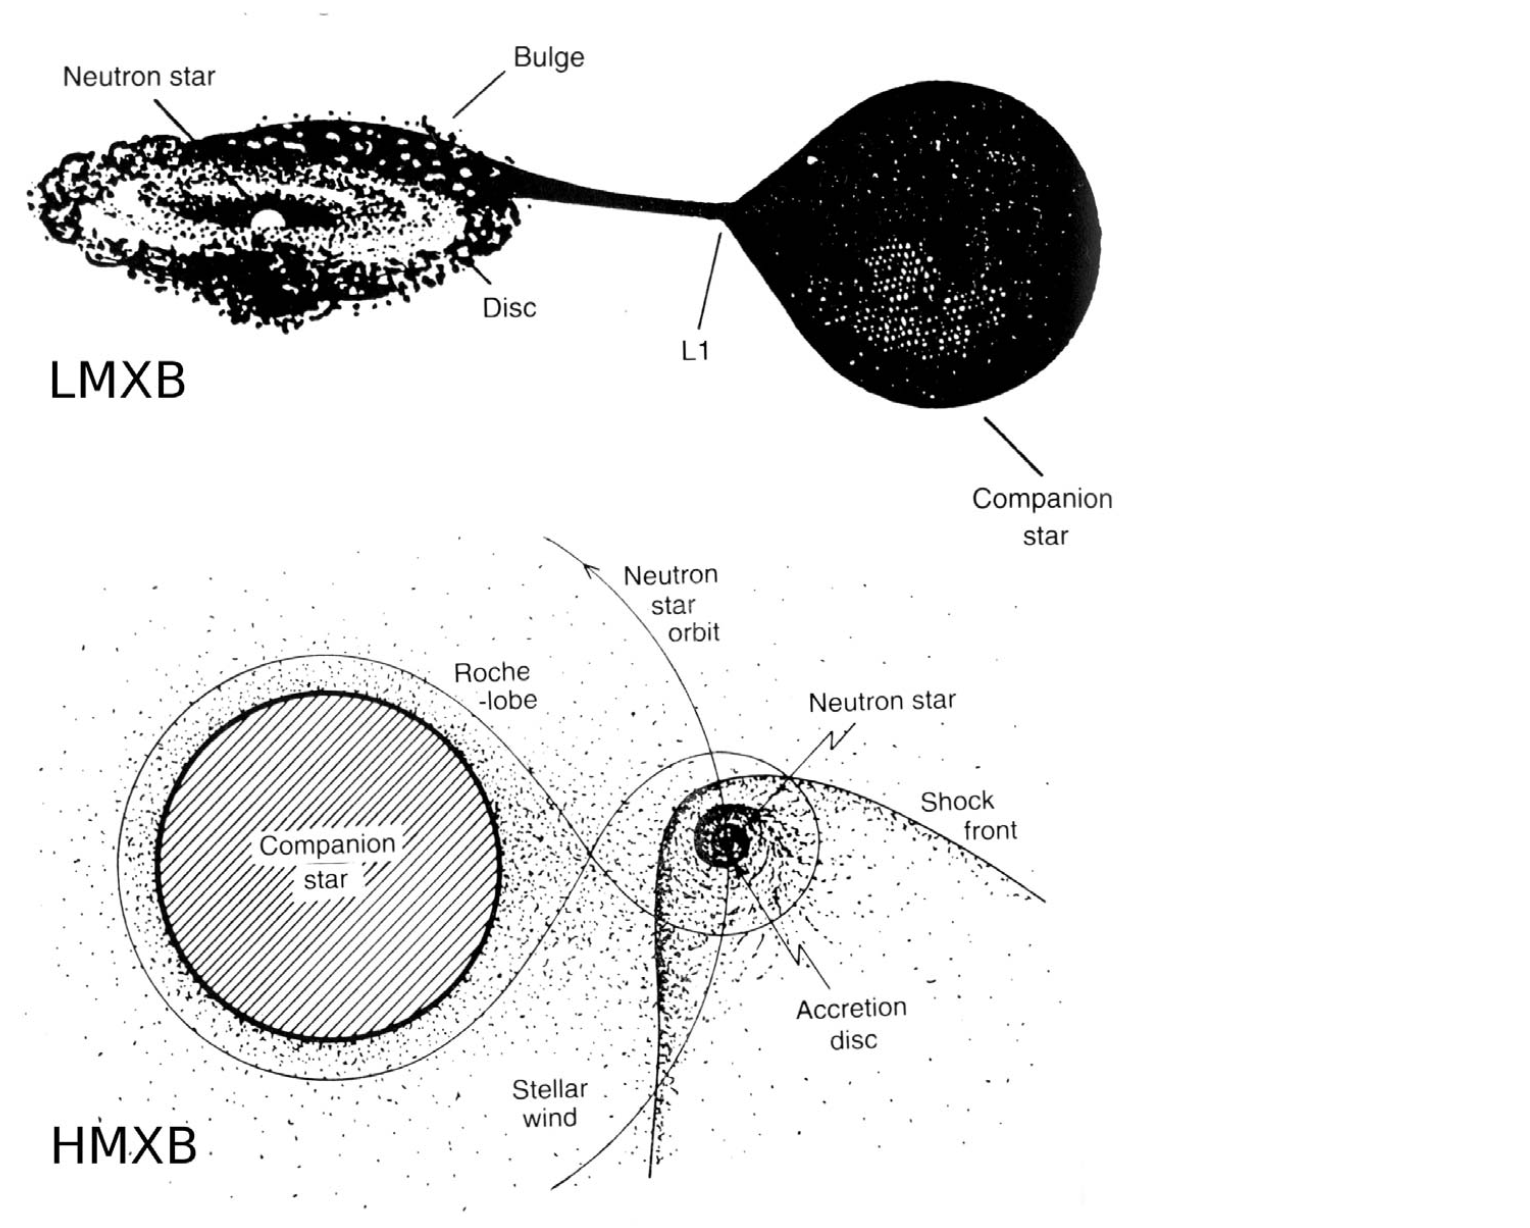
\includegraphics[width=1\linewidth]{Pictures/figures/hmxb_image.png}
    \caption{\small Artist’s conception of the two principal mechanisms by which matter is transferred onto a compact object in a binary
system. (top) A low-mass star has evolved and is losing mass to its degenerate companion because it fills its Roche lobe and mass
flows through the L 1 point. It is the presence of the compact object that distorts the mass-losing star into this shape (rather like a
pear), the vertex of which is the inner Lagrangian point, or L 1. Matter flowing out of the star forms a stream that impacts the
accretion disc (creating a bulge or thickened region) and, by viscous forces, is gradually accreted onto the compact object where
the X-rays are generated. The view is for binary phase 0.25. (bottom) The compact object is orbiting a massive star which has a
very powerful stellar wind – so powerful that there is sufficient material being lost in all directions for the compact object to
accrete and produce copious X-rays as it ploughs through this wind, thereby creating a comet-shaped shock front. The accretion
disc is small, and so fluctuations in wind density are immediately evident in the X-ray flux and pulsar frequency (courtesy EXOSAT
Observatory, ESA). (Taken from \textit{Exploring the X-ray Universe}.)}
    \label{fig:hmxb_image}
\end{figure}

High-mass X-ray binaries (HMXBs) are systems in which a compact object---typically a neutron star or a black hole---accretes material from a \textbf{massive, early-type companion star.} The donor is generally an O- or B-type star, often with masses $M_\ast \gtrsim 10\,M_\odot$, characterized by \textbf{strong stellar winds and high luminosities}. These winds provide the principal channel of mass transfer, distinguishing HMXBs from their low-mass counterparts, where \textbf{Roche-lobe overflow dominates}.

\subsection{Basic Properties}

HMXBs are among the brightest X-ray sources in the sky, with typical X-ray luminosities in the range
\[
L_X \sim 10^{35} - 10^{38}~\mathrm{erg~s^{-1}},
\]
depending on the accretion rate and compact object type. The systems generally have short orbital periods,
\[
P_{\rm orb} \sim 1~\text{to}~100~\mathrm{days},
\]
set by the balance between \textbf{wind accretion efficiency and the evolutionary state of the massive donor}.  
\begin{remark}
    It is important not to forget that the \textbf{mass-period relations} which apply to LMXBs due to the RLO mechanism are \textbf{not applicable} to wind accretion systems.
\end{remark}

The stellar wind mass-loss rate from the donor is typically
\[
\dot{M}_{\rm wind} \sim 10^{-7} - 10^{-5}\,M_\odot~\mathrm{yr^{-1}},
\]
with terminal velocities of order
\[
v_\infty \sim 1000~\mathrm{km~s^{-1}}.
\]
Only a small fraction of this wind is gravitationally captured by the compact object.\textbf{ The Bondi–Hoyle–Lyttleton accretion rate is often used as an approximation}:
\[
\dot{M}_{\rm acc} \approx \frac{(G M_{\rm X})^2 \dot{M}_{\rm wind}}
{(v_{\rm rel}^2 + c_s^2)^{3/2} a^2},
\]
where $M_{\rm X}$ is the compact object mass, $v_{\rm rel}$ is the relative velocity between the compact object and the stellar wind, $c_s$ is the sound speed in the wind, and $a$ is the orbital separation. 
The corresponding accretion luminosity is
\[
L_X \simeq \frac{G M_{\rm X} \dot{M}_{\rm acc}}{R_{\rm X}},
\]
where $R_{\rm X}$ is the radius of the compact object. For neutron stars, this yields typical luminosities near $10^{36}$--$10^{37}~\mathrm{erg~s^{-1}}$.

\subsubsection{Types of HMXBs}

High-mass X-ray binaries are broadly divided into two major subcategories based on the evolutionary state of the donor star and the dominant accretion mechanism: \textbf{supergiant systems} and \textbf{Be/X-ray binaries}. A small number of systems occupy intermediate or peculiar states, but the majority fall into one of these two classes.

\paragraph{Supergiant Systems (SGXBs)}

In \textbf{supergiant X-ray binaries} (SGXBs), the donor is an evolved O or B supergiant with a dense, radiatively driven \textbf{stellar wind}. The compact object---usually a neutron star---\textbf{accretes directly from this wind rather than through Roche-lobe overflow.} Because the accretion flow is highly inhomogeneous, these systems exhibit pronounced stochastic variability on short timescales, as well as periodic modulation with the orbital phase due to varying line-of-sight absorption.
\par
Typical parameters include:
\[
P_{\rm orb} \sim 1\text{--}10~\mathrm{days}, \quad
\dot{M}_{\rm wind} \sim 10^{-6}\,M_\odot~\mathrm{yr^{-1}}, \quad
L_X \sim 10^{36}\text{--}10^{37}~\mathrm{erg~s^{-1}}.
\]
\textbf{The X-ray luminosity is relatively steady compared to Be systems}, reflecting continuous wind capture. 
The X-ray spectrum is typically hard and highly absorbed, often displaying fluorescence features such as Fe~K$\alpha$, as well as cyclotron resonance scattering features (CRSFs) in neutron star systems, revealing the surface magnetic field strength ($B \sim 10^{12}$~G).  
\par
Some SGXBs are also \textbf{eclipsing binaries}, enabling precise dynamical mass measurements (e.g., Vela~X-1, 4U~1700$-$37, and Cyg~X-1). Others, termed \emph{supergiant fast X-ray transients (SFXTs)}, display sporadic outbursts \textbf{likely triggered by the capture of dense clumps within the stellar wind,} leading to rapid X-ray flares lasting hours to days.

\paragraph{Be/X-ray Binaries (BeXBs)}
In contrast, \textbf{Be/X-ray binaries} consist of a neutron star orbiting a rapidly rotating B-type star that possesses an equatorial \textbf{decretion disk} of gas ejected by the star’s high rotational velocity. The compact object follows a wide and often eccentric orbit ($P_{\rm orb} \sim 10$--$300~\mathrm{days}$), accreting only when it passes near periastron and interacts with the Be star’s disk. 
\par
As a result, BeXBs are typically \textbf{transient systems}, exhibiting two classes of outbursts:
\begin{itemize}
    \item \textbf{Type~I outbursts:} Regular, moderate-luminosity ($L_X \sim 10^{36}~\mathrm{erg~s^{-1}}$) events near periastron passage.
    \item \textbf{Type~II outbursts:} Giant, irregular events ($L_X \gtrsim 10^{37}~\mathrm{erg~s^{-1}}$) caused by large-scale disruptions or expansions of the Be decretion disk.
\end{itemize}

The optical spectra of Be donors are \textbf{characterized by strong Balmer emission lines (particularly H$\alpha$), arising from the circumstellar disk.} The double-peaked line profiles reflect Keplerian rotation in the disk and often vary with time as the disk grows or dissipates. These emission features both diagnose the disk dynamics and complicate radial velocity measurements.
\par
Most BeXBs host \textbf{X-ray pulsars}, where the neutron star’s strong magnetic field channels accreting material onto magnetic poles, producing pulsations with spin periods $P_{\rm spin} \sim 1$--$1000$~s. The systems show a broad correlation between orbital and spin period (the ``Corbet diagram''), reflecting the balance between wind torque and magnetospheric accretion.

\paragraph{Other and Transitional Systems}

A few systems exhibit hybrid characteristics or represent later evolutionary stages:
\begin{itemize}
    \item \textbf{Roche-lobe overflow HMXBs:} Very rare, short-period systems in which the massive donor fills its Roche lobe and drives persistent disk accretion (e.g., LMC~X-4).
    \item \textbf{Wolf–Rayet binaries:} Extremely evolved donors with powerful, helium-rich winds feeding a compact companion (e.g., Cyg~X-3).
\end{itemize}

\par
In summary, HMXB subtypes trace different stages of massive binary evolution and reveal distinct accretion physics. SGXBs probe quasi-spherical wind accretion and radiative feedback, while BeXBs highlight transient disk-fed accretion and magnetically channeled flows. Together, they form the dominant population of X-ray binaries in young stellar environments and provide essential constraints on compact object formation and binary evolution pathways.

\subsubsection{Localization of HMXBs}

High-mass X-ray binaries are found \textbf{predominantly in regions of active or recent star formation}, reflecting the short lifetimes of their massive stellar companions. Since O- and B-type stars evolve on timescales of only a few million years, HMXBs trace the \emph{young stellar population} of a galaxy. Their spatial distribution therefore offers strong evidence that they are short-lived evolutionary phases in the lives of massive binaries.

\par
Within the Milky Way, HMXBs are concentrated along the Galactic plane and particularly near the spiral arms, coinciding with sites of ongoing star formation such as OB associations and H\,\textsc{ii} regions. This localization is consistent with the fact that their progenitor binaries form and evolve rapidly before the massive star undergoes core collapse. The compact object (a neutron star or black hole) forms in a supernova, and if the binary survives the explosion, it remains close to its birthplace.
\par
Because of these youth and kinematic properties:
\begin{itemize}
    \item HMXBs are often located within a few hundred parsecs of star-forming complexes or molecular clouds.
    \item They exhibit moderate space velocities ($\sim 10$--$100~\mathrm{km~s^{-1}}$), potentially imparted by the supernova kick, but not sufficient to carry them far from their birth sites.
    \item Their vertical scale height above the Galactic plane is small ($z \lesssim 200$~pc), consistent with Population~I objects.
\end{itemize}
\par
In contrast, \textbf{low-mass X-ray binaries (LMXBs)} show a completely different spatial distribution. Their old, low-mass donors imply long evolutionary timescales, allowing them to migrate far from their birthplaces. Consequently, LMXBs are found throughout the Galactic bulge and halo, and many are associated with \textbf{globular clusters}. Their high scale heights ($z \sim 1$--$2$~kpc) reflect their membership in the old stellar population.
\par
The differing localizations of HMXBs and LMXBs therefore trace the star-formation history of galaxies: 
HMXBs mark \textbf{young, massive stellar environments}, while LMXBs trace the \textbf{ancient, dynamically evolved populations}. In external galaxies, this distinction manifests as a strong correlation between HMXB number and recent star-formation rate, and between LMXB number and total stellar mass.

\subsubsection{Accretion Mechanisms}

In high-mass X-ray binaries, accretion proceeds primarily through the capture of the \textbf{stellar wind} from the massive companion. The strong, radiatively driven wind of an O/B supergiant provides a continuous outflow of material that the compact object can gravitationally capture. This process is well described by the \textbf{Bondi–Hoyle–Lyttleton (BHL) accretion model}, in which the compact object effectively sweeps up a fraction of the stellar wind as it moves through it.

\par
The mass accretion rate is approximately
\[
\dot{M}_{\rm acc} \approx \pi R_{\rm acc}^2 \rho v_{\rm rel},
\qquad
R_{\rm acc} = \frac{2 G M_{\rm X}}{v_{\rm rel}^2 + c_s^2},
\]
where $R_{\rm acc}$ is the accretion radius, $\rho$ is the local wind density, $v_{\rm rel}$ is the relative velocity between the compact object and the wind, and $c_s$ is the sound speed. Only a small portion of the stellar wind is accreted, but given the high wind mass-loss rates, this is sufficient to generate X-ray luminosities of $L_X \sim 10^{36}$--$10^{37}~\mathrm{erg~s^{-1}}$.

\par
As the accreted material approaches the compact object, it encounters the \textbf{magnetosphere} of the neutron star. At the \textbf{magnetospheric radius} $R_{\rm m}$, the magnetic pressure balances the ram pressure of the inflowing gas. Inside this radius, the magnetic field dominates the flow dynamics, forcing the plasma to follow magnetic field lines and funneling it toward the magnetic poles. 

\par
At the neutron star surface, the inflow decelerates in a strong shock, forming a localized \textbf{accretion column} where kinetic energy is converted into thermal and radiative energy. The resulting hot spots emit primarily in X-rays, with characteristic luminosities up to $\sim 10^{38}~\mathrm{erg~s^{-1}}$. If the magnetic axis is \textbf{misaligned with the rotation axis}, the emission appears modulated at the stellar spin period, producing the characteristic \textbf{X-ray pulsar} phenomenon. These pulsations directly probe the rotation rate, magnetic field structure, and accretion geometry of the compact object.

\par
In contrast, \textbf{Be/X-ray binaries} operate through a different, highly variable accretion mode. The Be donor possesses a dense, equatorial \textbf{decretion disk} of gas expelled by rapid rotation. The compact object, typically in an eccentric orbit, captures material from this disk primarily during periastron passages. The interaction triggers episodic accretion events and consequent X-ray outbursts. 

\par
Two types of outbursts are typically observed:
\begin{itemize}
    \item \textbf{Type~I outbursts:} Modest, periodic events ($L_X \sim 10^{36}~\mathrm{erg~s^{-1}}$) occurring near periastron.
    \item \textbf{Type~II outbursts:} Bright, irregular outbursts ($L_X \gtrsim 10^{37}~\mathrm{erg~s^{-1}}$), associated with large-scale expansions or instabilities in the Be disk.
\end{itemize}

\par
In both wind-fed and Be-fed systems, the details of accretion---including angular momentum capture, magnetic coupling, and radiative feedback---play key roles in setting the X-ray luminosity and variability. Together, these mechanisms underpin the rich phenomenology of HMXBs, linking stellar winds, magnetospheric physics, and high-energy radiation in a unified framework.

\subsection{HMXBs as Spectroscopic Binaries}

Since the O/B-type companion in a high-mass X-ray binary is extremely \textbf{luminous}, we can generally observe both the emission from the accretion process (\textbf{X-ray radiation}) and the emission from the massive companion (\textbf{optical/UV continuum}). This dual visibility makes HMXBs \textbf{double-lined spectroscopic binaries}, allowing dynamical studies of both components and, consequently, direct constraints on the compact object mass.

\par
The donor star’s spectrum is dominated by its photospheric absorption lines (H~I, He~I, He~II, and various metallic features). However, the presence of the compact object and its energetic radiation field substantially alters the observed optical spectrum. X-ray photoionization of the stellar wind and reprocessing in the accretion flow introduce strong \textbf{emission components}---particularly in the Balmer series (most notably H$\alpha$), He~II~$\lambda4686$, and sometimes Fe~II and N~III lines. These can \textbf{partially fill in} or even \textbf{reverse} the absorption features, leading to distorted or asymmetric line profiles. The resulting composite spectrum often varies with orbital phase, reflecting changes in the ionization structure of the stellar wind and accretion wake. Even in the optical, this can produce a veiling of the photospheric lines, complicating radial velocity measurements and spectral classification.

\par
In systems hosting neutron stars, \textbf{X-ray pulsations} provide a direct tracer of the compact object’s orbital motion. In others, Doppler shifts in X-ray or emission-line features from the accretion flow can be used to extract the compact object’s velocity amplitude $K_{\rm X}$. Meanwhile, the O/B star’s optical spectrum traces its own motion with velocity amplitude $K_\ast \sim 10$--$100~\mathrm{km~s^{-1}}$. The ratio of these amplitudes yields the binary mass ratio:
\[
\frac{M_{\rm X}}{M_\ast} = \frac{K_\ast}{K_{\rm X}}.
\]
Combining this ratio with the orbital period $P_{\rm orb}$ provides the \textbf{standard mass function,}
\[
f(M) = \frac{(M_{\rm X} \sin i)^3}{(M_\ast + M_{\rm X})^2}
= \frac{P_{\rm orb} K_\ast^3}{2\pi G},
\]
which sets a firm \emph{lower bound} on the \textbf{mass of the compact object.} For eclipsing systems, where the inclination $i$ can be accurately determined ($i \gtrsim 75^\circ$), both $M_{\rm X}$ and $M_\ast$ can be measured directly with relatively small uncertainties.

\par
Spectroscopic complications are especially pronounced in supergiant systems, where dense winds and strong X-ray irradiation produce extended emission-line regions, and in Be/X-ray binaries, where the Be star’s decretion disk gives rise to variable, double-peaked Balmer emission lines. These effects must be carefully modeled to disentangle stellar, disk, and wind contributions. Nonetheless, the ability to observe both components spectroscopically makes HMXBs among the most powerful laboratories for constraining compact object masses and testing models of binary evolution.

\subsection{Observational Diagnostics}

High-mass X-ray binaries display a wide range of \textbf{observational signatures} that reveal the complex interplay between accretion, radiation, and stellar winds. Their variability spans timescales from seconds to years and offers a powerful window into the geometry and dynamics of the accretion process. 

\par
A defining feature of HMXBs is their \textbf{orbital modulation} of X-ray flux. As the compact object traverses the dense stellar wind of its massive companion, the line-of-sight column density varies periodically, leading to strong changes in observed brightness. In many systems, this modulation is further enhanced by geometric \textbf{eclipses}, during which the donor star partially or completely obscures the X-ray source. Because the absorbing material contains metals, the increased column density preferentially extinguishes soft X-rays, producing phase-dependent changes in the continuum shape. Even in deeply eclipsing systems, however, \textbf{radiative transfer and photoionization} within the wind ensure that emission lines remain visible, as they originate from extended regions of ionized gas rather than from the compact source itself.

\par
Another characteristic signature arises from \textbf{X-ray pulsations}, observed in systems hosting magnetized neutron stars. In these binaries, the accreting material is funneled along magnetic field lines onto the neutron star’s magnetic poles, forming localized hot spots. As the neutron star rotates, the anisotropic emission from these poles produces coherent pulsations, with periods ranging from $\sim 1$ to $1000$~s. The pulse profiles and their energy dependence provide valuable constraints on the geometry of the accretion column and the strength and configuration of the magnetic field.

\par
In addition to these periodic signals, HMXBs exhibit a rich variety of \textbf{long-term and aperiodic variability}. Changes in the density and structure of the stellar wind can modulate the accretion rate on timescales of weeks to months, while in Be/X-ray binaries, the quasi-cyclic formation and dissipation of the Be star’s decretion disk drive recurring outbursts and extended quiescent phases. Some systems show distinct \textbf{spectral state changes}, transitioning between high- and low-luminosity states that are often accompanied by variations in hardness ratio. These transitions typically trace fluctuations in the accretion rate or shifts in the absorbing column along the line of sight.

\par
Spectroscopically, HMXBs display \textbf{complex and diagnostic X-ray spectra} that encode the physical properties of the accretion environment. The continuum emission is generally hard, arising from \textbf{thermal bremsstrahlung} or \textbf{Comptonized emission} within the accretion column or corona. Superimposed on this continuum are strong spectral features, most notably the \textbf{Fe~K$\alpha$ fluorescence line} at 6.4~keV, which originates from reprocessing in cool, dense material near the compact object. Additional photoionization and recombination lines reveal the presence of extended, partially ionized gas in the stellar wind. Many systems also exhibit \textbf{energy-dependent absorption}, with partial-covering models required to explain spectra affected by dense or clumpy winds. These absorption effects frequently produce sharp low-energy cutoffs and variable attenuation of the continuum flux.

\par
Taken together, these timing and spectral diagnostics make HMXBs uniquely valuable laboratories for studying accretion under extreme conditions. They provide empirical constraints on wind-fed accretion, magnetic channeling, and radiative feedback, linking the physics of massive stars to the high-energy behavior of compact objects in binary systems.



\subsection{Spectroscopic Features}

The composite spectra of high-mass X-ray binaries reflect contributions from both the massive donor star and the compact accretor, as well as their mutual interaction through winds and radiation. Each component imprints distinct features across the electromagnetic spectrum.

\subsubsection{Stellar and Wind Signatures}

The \textbf{optical and UV spectra} are dominated by the massive O/B-type donor, which exhibits strong photospheric absorption lines (H~I, He~I, He~II, and various metal lines). However, X-ray irradiation and the presence of a dense, structured stellar wind significantly modify these features:
\begin{itemize}
    \item Reprocessing in the wind produces prominent \textbf{emission lines}, particularly H$\alpha$, He~II~$\lambda4686$, and Fe~II multiplets, which can partially fill in or even reverse absorption features.
    \item The stellar wind is highly \textbf{clumpy and anisotropic}, giving rise to stochastic variability and asymmetric line profiles that vary with orbital phase. This was found by \citet{1999ApJ...525..921S} based on the presence of spectroscopic signatures from both cold gas and photoionized gas suggesting inhomogeneity.
    \item In Be/X-ray binaries, the decretion disk adds strong, often double-peaked Balmer emission lines tracing Keplerian rotation in the disk.
\end{itemize}

\subsubsection{X-ray Spectral Features}

The \textbf{X-ray emission} arises primarily from hot, shocked plasma near the compact object. The continuum is typically a power law with an exponential cutoff above $\sim 10$--$30$~keV, consistent with \textbf{thermal bremsstrahlung} or \textbf{Comptonized emission} from the accretion column or corona. Superimposed on this continuum are:
\begin{itemize}
    \item \textbf{Emission lines} from highly ionized species (e.g., Fe~XXV, Fe~XXVI), produced by photoionization in the stellar wind.
    \item The ubiquitous \textbf{Fe~K$\alpha$ fluorescence line} at 6.4~keV, a key tracer of dense, neutral material near the compact object.
    \item Broad absorption features identified as \textbf{cyclotron resonance scattering features (CRSFs)}, which directly measure the magnetic field strength of the neutron star.
    \item Variable absorption edges and partial covering components, reflecting the inhomogeneous wind and orbital modulation of the column density.
\end{itemize}

\subsubsection{Eclipsing and Reprocessing Effects}

In \textbf{eclipsing HMXBs}, the optical star can completely block the direct continuum X-ray emission when the compact object passes behind it. During such eclipses, the observed spectrum becomes dominated by \textbf{scattered and reprocessed emission} originating in the extended stellar wind and circumstellar gas. Remarkably, while the continuum flux drops dramatically, the emission lines remain largely unchanged, since they are produced in photoionized gas on scales much larger than the stellar radius.

\par
This behavior allows observers to isolate the reprocessed emission and study the ionization structure and density of the surrounding medium, providing a natural laboratory for testing radiative transfer and wind models in high-energy astrophysical environments.


\subsection{Evolution of HMXBs}
\begin{figure}
    \centering
    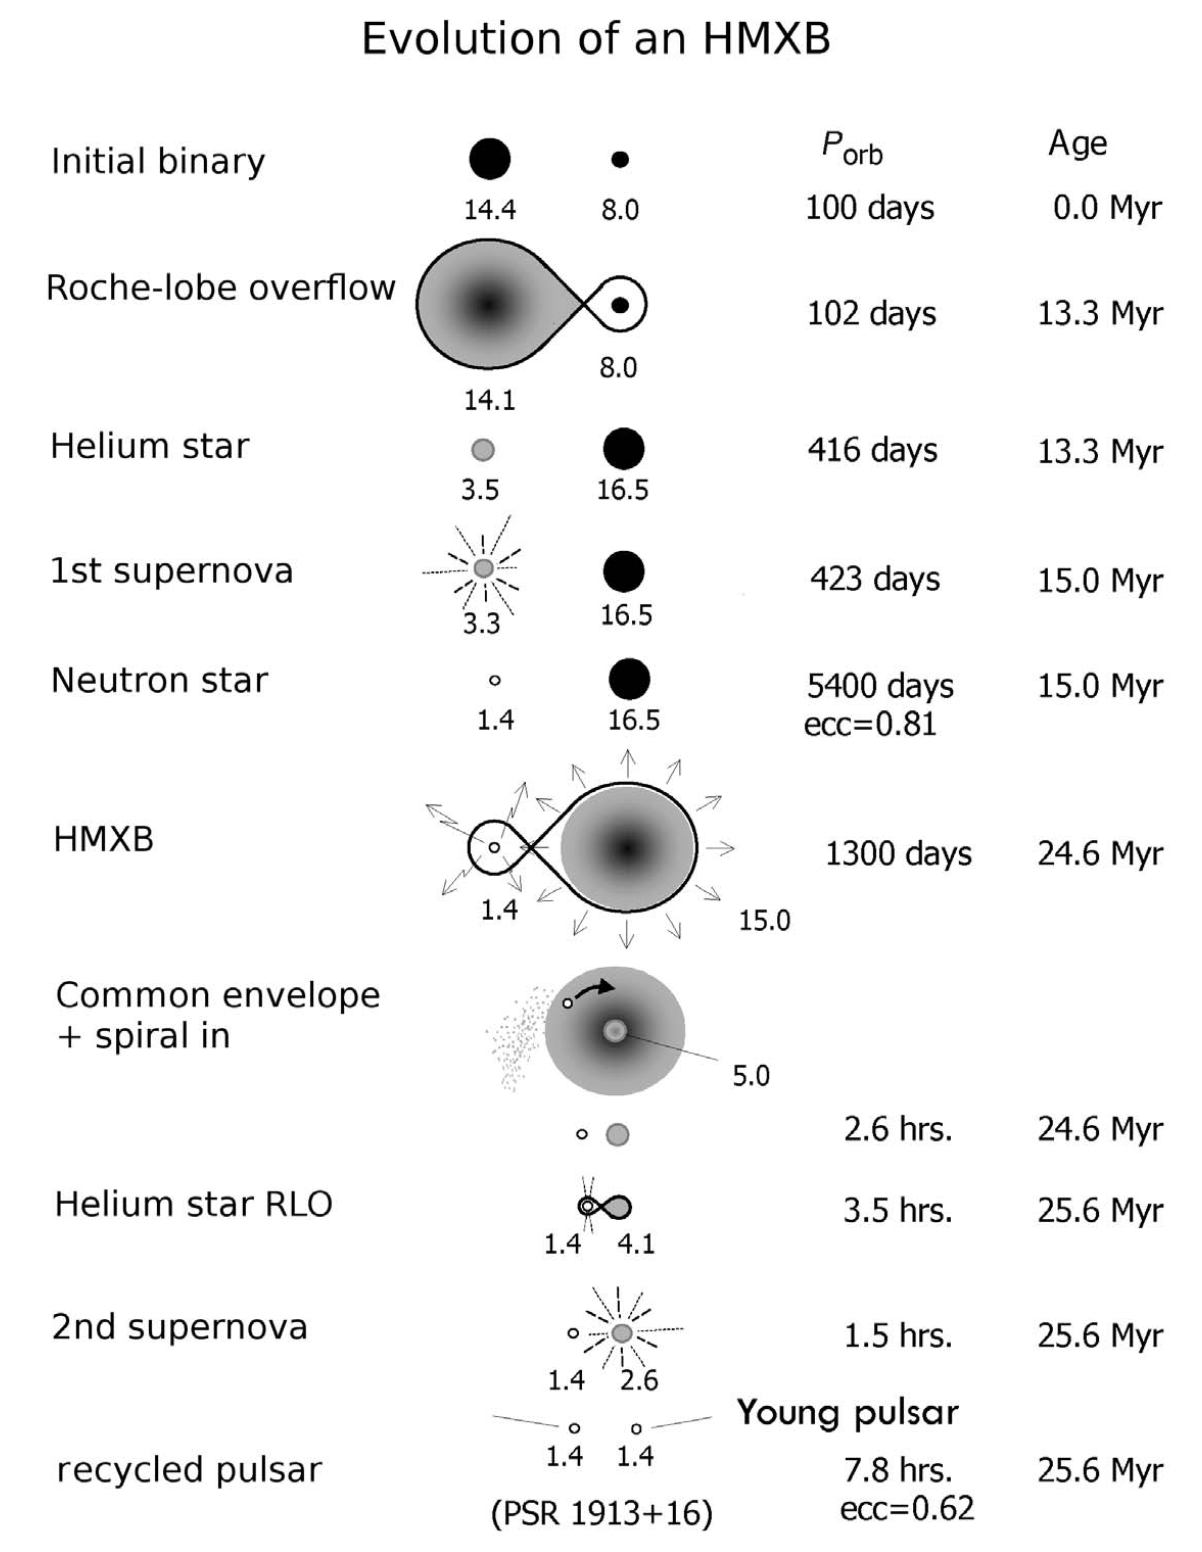
\includegraphics[width=1\linewidth]{Pictures/figures/hmxb_evol.png}
    \caption{Evolutionary scenario for the formation of an HMXB/Be star from an initial binary of two stars of differing large mass
at age 0. The more massive star evolves fastest, producing the first supernova event after 15 Myr. The resulting neutron star leads
to the HMXB/Be phase once the surviving star has itself evolved to become a giant. This phase does not last long, and following a
common-envelope ‘spiral-in’, a second supernova event can lead to the formation of a binary pulsar system (diagram based on
Tauris \& van den Heuvel, 2006). (Taken from \textit{Exploring the X-ray Universe}.)}
    \label{fig:hmxb_evolution}
\end{figure}
The canonical formation path for a high-mass X-ray binary proceeds through a sequence of short-lived but observationally supported stages. A representative example begins with a massive binary (orbital period $\sim$100~days) in which the initially \emph{more massive} primary evolves rapidly, expands, and fills its Roche lobe after $\sim 13$~Myr, initiating the \textbf{first mass-transfer episode}. In the illustrative case shown, $\sim 9\,M_\odot$ are transferred to the companion in $\sim 5\times10^4$~yr, leaving a $\sim 3.5\,M_\odot$ helium core and widening the orbit to $\gtrsim 400$~days due to mass and angular-momentum exchange.
\rmk{Remember, we are transferring from the more massive primary to the less massive secondary, which means the orbit will expand.}
\paragraph{Helium-star (Wolf–Rayet) phase and the first supernova.}
After envelope stripping, the primary is observed as a helium (Wolf–Rayet) star whose energy source is helium fusion; within $\sim 2$~Myr it undergoes \emph{the first core-collapse supernova}. The prompt mass loss and explosion asymmetry typically yield a highly eccentric, longer-period post-SN orbit—and often disrupt the binary entirely, a fact that helps explain the rarity of X-ray binaries.

\paragraph{The HMXB phase.}
If the binary survives, the compact remnant (usually a neutron star) orbits the still-massive secondary. While that secondary remains an O/B star, wind-fed accretion powers the \emph{HMXB} episode; \textbf{this phase is comparatively brief in population terms}. As the donor later evolves and \emph{expands}, mass transfer becomes dynamically unstable (for extreme mass ratios, $q\!=\!M_{\rm donor}/M_{\rm acc}\!\gg\!1$), leading to \emph{common-envelope (CE) evolution}: friction in the shared envelope removes orbital energy and angular momentum, driving a spiral-in. The outcome is a dramatic period shrinkage to hours and ejection of the donor’s H-rich envelope, leaving a tight neutron-star + helium-star system. For context on stability: Roche-lobe overflow is \emph{only} stably maintained when the donor is \emph{less} massive than the accretor; when the donor is more massive (as in this stage) instability and CE are expected.

\paragraph{Roche-lobe overflow from the helium star and the second supernova.}
In the post-CE binary, the stripped helium star can subsequently \emph{overflow its Roche lobe} and transfer mass onto the neutron star in a short-period orbit, before ultimately undergoing a \emph{second} supernova. A surviving system emerges as a \emph{double neutron star}—as exemplified by radio pulsar binaries such as PSR~1913+16—providing striking observational evidence for this evolutionary channel. 

\paragraph{Link to star-formation history.}
Because HMXB lifetimes are short, their numbers and luminosity functions \emph{track recent star formation}. The pronounced overabundance of HMXBs in the SMC is explained by a $\sim 100$~Myr-old interaction-triggered starburst, and across external galaxies the cumulative HMXB luminosity functions align when scaled by the star-formation rate, making HMXBs effective SFR indicators.

\subsection{Relativistic Jets}
- The blue jet and the optical jet are not quite the same. Unclear why? 
- The relativistic jets and the kinetic view of them -> how we use SR to get the velocities due to transverse doppler shift.

\section{The Nature of the Accretor}

\begin{figure}[ht!]
    \centering
    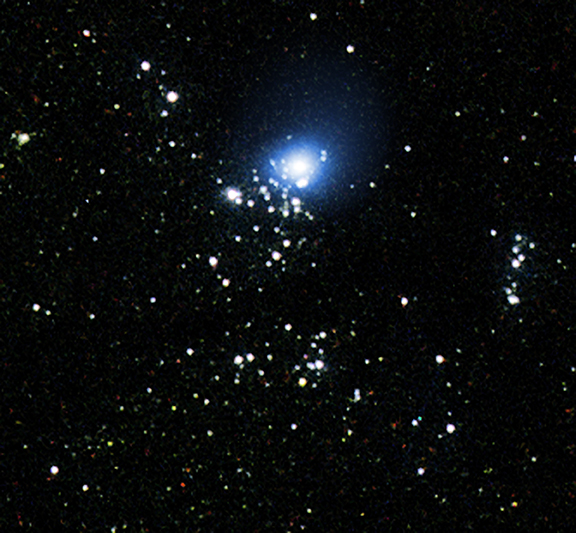
\includegraphics[width=0.5\linewidth]{Pictures/figures/x-7.png}
    \caption{The composite image includes data from NASA's Chandra X-ray Observatory (blue) and the Hubble Space Telescope. The bright objects in the inset image are young, massive stars around M33 X-7, and the bright, blue Chandra source is M33 X-7 itself. X-rays from Chandra reveals how long the black hole is eclipsed by the companion star, which indicates the size of the companion. }
\end{figure}

Once an X-ray binary is identified, a fundamental question arises: is the compact object accreting matter a neutron star or a black hole? Since black holes emit no light themselves, their presence must be inferred gravitationally. The definitive discriminant is mass. Theory and observation place a firm upper limit on the mass of a stable neutron star, known as the Tolman-Oppenheimer-Volkoff limit, at approximately $3 M_{\odot}$. Any compact object with a dynamically measured mass that conclusively exceeds this threshold cannot be a neutron star and is therefore considered a black hole.

Low-Mass X-ray Binaries (LMXBs) have proven to be the most fertile ground for finding and weighing stellar-mass black holes. The low mass of the companion star means that any measurement of the system's total mass is dominated by the compact object, providing a cleaner result. Crucially, the long quiescent periods of transient LMXBs are a gift to observers; with the accretion disk dormant and faint, the light from the faint companion star can be isolated and studied in detail to precisely measure its orbital parameters.

The primary tool for this task is the \textbf{mass function}, derived from observing the spectral lines of the visible companion star in what is known as a single-lined spectroscopic binary. By measuring the star's orbital period ($P$) and the amplitude of its radial velocity ($K_c$), one can calculate the mass function, $f(M)$:

\[
f(M) = \frac{P K_c^3}{2\pi G} = \frac{(M_X \sin i)^3}{(M_X + M_c)^2}
\]

where $M_X$ and $M_c$ are the masses of the compact object and companion, respectively, and $i$ is the orbital inclination. The value $f(M)$ provides an absolute minimum mass for the compact object ($f(M) \leq M_X$). Several LMXBs have mass functions well in excess of $3 M_{\odot}$, providing unambiguous proof of a black hole.

While LMXBs are ideal, the most "gold-standard" confirmations can come from rare systems with special geometries. A prime example is \textbf{M33 X-7}, a High-Mass X-ray Binary that happens to be an \textbf{eclipsing} system. The presence of deep eclipses tells us that we are viewing the orbit almost perfectly edge-on ($i \approx 90^{\circ}$), which eliminates the main uncertainty in the mass function since $\sin i \approx 1$. With the inclination constrained, the mass of the accretor was precisely measured to be $15.65 \pm 1.45 M_{\odot}$. This value is more than five times the maximum possible mass of a neutron star, making M33 X-7 one of the most securely identified black holes known.